% -*- root: article.tex -*-
O \emph{objetivo} deste estudo é investigar boas e más práticas no desenvolvimento do \textit{front-end} Android. Portanto, conduzimos um estudo qualitativo e exploratório no qual coletamos dados através de dios questionários online com desenvoveldores Android. O primeiro questionário (\textit{S1}) teve foco em investigar boas e más práticas no desenvolvimento Android. O segundo questionário (\textit{S2}) teve foco em avaliar a percepção dos desenvolvedores sobre as más práticas definidas a partir de \textit{S1}. 

\mau{defenda aqui o uso de estudos qualitativos, veja como Michaela Greiler fez 'test confessions'}

Esta seção descreve de forma detalhada a estrutura dos questionários, os participantes e as análises realizadas sobre as respostas obtidas.

\subsection{Boas e Más Práticas Android}

Para responder a \textbf{QP1}, buscamos entender o que desenvolvedores consideram boas e más práticas no desenvolvimento do \textit{front-end} Android. Os dados foram coletados através de um questionário online (\textit{S1}) respondido por 45 desenvolvedores. Realizamos um processo de codificação aberta sobre os dados, resultando num conjunto com 23 categorias de boas e más práticas Android. Estas categorias foram agrupadas de acordo com sua recorrência nas respostas, ou seja, a quantidade de respostas que determinada categoria é percebidas, quanto mais respostas, maior a recorrência.

\subsubsection{Questionário}
\label{sub:questionario}

O questionário continha 25 questões divididas em três seções. A primeira seção continha 6 perguntas demográficas, a segunda seção continha 16 perguntas sobre boas e más práticas relacionadas ao \textit{front-end} Android e a terceira seção continha 3 perguntas, 2 para obter últimos pensamentos sobre boas e más práticas e 1 solicitando email caso o participante tivesse interesse em etapas futuras da pesquisa. O questionário foi escrito em inglês porém informava o participante que respostas em inglês ou português eram aceitas. Antes da divulgação, realizamos um piloto com 3 desenvolvedores Android. Todos estes dados estão disponíveis em nosso pacote de replicação\footnote{https://github.com/SuelenGC/android-code-smells-article}.

\mau{mencionar em algum lugar que as perguntas eram opcionais, e explicar o pq.}

A primeira seção continha 6 questões demográficas obrigatórias de multipla escolha. Abordavam sobre idade (18 ou menos, 19 a 24, 25 a 34 e assim por diante até 55 ou mais), estado de residência (foi dada uma lista com estados do Brasil, Estados Unidos e Europa), anos de experiência com desenvolvimento de software, (1 anos ou menos, 2 anos, 3 anos, e assim por diante até 10 ou mais), anos de experiência com desenvolvimento Android (mesma escala de anos da questão anterior), uma questão sobre linguagens que o participante se considerava proeficiente (Java, Python, Ruby, Android, dentre outras) e sobre o último grau de escolaridade (estudante de bacharelado, bacharel, mestrado e doutorado). As questões sobre idade, região, linguagens e grau de escolaridade continham a opção ``outros'' para o caso de nenhuma das opções atenderem, ao selecionar ``outros'' era possível escrever uma resposta.

A segunda seção continha 16 questões opcionais e dissertativas sobre boas e más práticas relacionadas ao \textit{front-end} Android. Para cada elemento do \textit{front-end} Android foram feitas duas perguntas, uma sobre boas e outra sobre más práticas percebidas pelos participantes. Por exemplo, para o elemento \textsc{Activity} foram feitas as seguintes perguntas: \\

\noindent
\textbf{Q1} Você tem alguma boa prática para lidar com Activities? (Resposta aberta) \\

\noindent
\textbf{Q2} Você considera alguma coisa uma má prática ao lidar com Activities? (Resposta aberta) \\

A terceira seção continha 3 perguntas opcionais e dissertativas, 2 para captar qualquer última ideia sobre boas e más práticas não captadas nas questões anteriores e 1 solicitando o email do participante caso o mesmo tivesse interesse em participar de etapas futuras da pesquisa. 

Antes da divulgação, realizamos um piloto com 3 desenvolvedores Android e com o feedback deles fizemos alguns ajustes relacionados a obrigatoriedade das perguntas da segunda seção do questionário, onde todas tornaram-se opcionais. As respostas dos participantes piloto foram desconsideradas para efeitos de viés. 

% Todas as 18 questões sobre boas e más práticas (16 na segunda seção e 2 da terceira) são apresentadas na Tabela \ref{tab:RespostasXParticipantes}.

% \begin{table*}[t]
% \centering
% \footnotesize
% \begin{tabular}{@{}lp{8.5cm}ccp{6cm}@{}}
% \toprule
% \multirow{2}{*}{\textbf{Id}}& \multicolumn{1}{c}{\multirow{2}{*}{\textbf{Questões}}} 	& \multicolumn{2}{c}{\textbf{Respostas}}	& \multicolumn{1}{c}{\multirow{2}{*}{\textbf{Participantes}}} \\ \cmidrule{3-4}
% 					 		& 															& \textbf{Total} & \textbf{\%} & \\
% \hline
% Q1	& Você tem alguma boa prática para lidar com Activities?															&36 &80\%	&P1, P2, P4--P12, P14--P17, P19, P22, P23, P25--P32, P34--P37, P39--P43, P45 \\
% Q2	& Você considera alguma coisa uma má prática ao lidar com Activities?									&35 &78\%	&P2, P4--P11, P14--P17, P19, P22, P23, P25--P32, P34--P37, P39--P45 \\
% Q3	& Você tem alguma boa prática para lidar com Fragments?															&33	&73\%	&P4--P11, P14--P17, P19, P22, P23, P25--P28, P30--P32, P34--P37, P39--P45 \\
% Q4	& Você considera alguma coisa uma má prática ao lidar com Fragments?										&31	&69\%	&P2, P4--P11, P14, P15, P17, P19, P22, P23, P25--P28, P31,P32, P34--P37, P39--P43, P45 \\
% Q5	& Você tem alguma boa prática para lidar com Adapters?																&30	&67\%	&P2, P4--P11, P14, P15, P17--P19, P22, P23, P26, P28, P29, P31,P32, P34--P37, P39--P43, P45 \\
% Q6	& Você considera alguma coisa uma má prática ao lidar com Adapters?										&27	&60\%	&P2, P4--P8, P10, P11, P14, P18, P19, P22, P23, P26, P28, P31, P34--P37, P39--P45 \\
% Q7	& Você tem alguma boa prática para lidar com Listeners?															&24	&53\%	&P2, P4--P6, P8, P9, P11, P14, P22, P23, P26, P28, P29, P31, P32, P34, P36, P37, P39--P43, P45 \\
% Q8	& Você considera alguma coisa uma má prática ao lidar com Listeners?										&23	&51\%	&P2, P4, P5, P8, P9, P11, P14, P19, P22, P23, P26, P28, P31, P32, P34, P36, P37, P39--P44 \\
% Q9	& Você tem alguma boa prática para lidar com Layout Resources?														&28	&62\%	&P4--P9, P11, P14, P19, P22, P23, P26--P29, P31, P32, P34--P37, P39--P45 \\
% Q10	& Você considera alguma coisa uma má prática ao lidar com Layout Resources?								&23	&51\%	&P4, P5, P7--P9, P11, P22, P23, P26, P28, P31, P32, P34--P37, P39--P45 \\
% Q11	& Você tem alguma boa prática para lidar com Styles Resources?														&23	&51\%	&P4--P9, P11, P18, P22, P23, P26, P28, P31, P32, P34--P37, P39--P43 \\
% Q12	& Você considera alguma coisa uma má prática ao lidar com Styles Resources?								&22	&49\%	&P4--P8, P11, P18, P22, P23, P26, P28, P31, P32, P34--P37, P39--P43 \\
% Q13	& Você tem alguma boa prática para lidar com String Resources?														&28	&62\%	&P4--P6, P8--P11, P14, P18, P22, P23, P26--P29, P31, P32, P34--P37, P39--P45 \\
% Q14	& Você considera alguma coisa uma má prática ao lidar com String Resources?								&23	&51\%	&P4--P6, P8, P9, P11, P14, P18, P22, P23, P26, P28, P31, P32, P34--P37, P40--P43, P45 \\
% Q15	& Você tem alguma boa prática para lidar com Drawable Resources?													&24	&53\%	&P4--P6, P8--P11, P14, P18, P22, P23, P26, P28, P31, P32, P34--P37, P39--P43 \\
% Q16	& Você considera alguma coisa uma má prática ao lidar com Drawable Resources?							&21	&47\%	&P4--P6, P8, P11, P14, P18, P22, P23, P26, P28, P31, P32, P34, P36, P37, P40--P44 \\
% Q17	& Existem outras *BOAS* práticas sobre a Camada de Apresentação Android que nós não perguntamos ou que você não disse ainda?	&22	&49\%	&P2, P4, P8, P10, P11, P14, P18, P22, P23, P26, P28, P31, P32, P34, P36, P37, P39--P43, P45 \\
% Q18	& Existem outras *MáS* práticas sobre a Camada de Apresentação Android que nós não perguntamos ou que você não disse ainda?	&20	&44\%	&P2, P4, P8, P10, P11, P18, P22, P23, P28, P31, P32, P34, P36, P37, P40--P45 \\
% \hline
% \multicolumn{5}{@{}l}{\textit{* Os participantes P3, P13, P20, P21, P24, P33 e P38 não responderam nenhuma das questões da segunda e terceira seção.}} \\
% \toprule
% \end{tabular}
% \caption{Total de respostas obtidas por cada questão sobre boas e más práticas no \textit{front-end} Android.}
% \label{tab:RespostasXParticipantes}
% \end{table*}

\subsubsection{Participantes}
\label{sub:participantes}


% \mau{a tabela 1 nao eh tao importante. vc pode coloca-la no apendice online. mencione que ela existe no apendice online.}

O questionário foi divulgado em redes sociais como Facebook, Twitter e Linkedin, em grupos de discussão sobre Android como \href{https://groups.google.com/forum/#!forum/androidbrasil-dev}{\textit{Android Dev Brasil}}, \href{https://groups.google.com/forum/\#!forum/android-brasil--projetos}{\textit{Android Brasil Projetos}} e o grupo do \href{http://slack.androiddevbr.org/}{\textit{Slack Android Dev Br}}, maior grupo de desenvolvedores Android do Brasil com 2622 participantes até o momento da escrita deste artigo. 
O questionário esteve aberto por aproximadamente 3 meses e meio, de 9 de Outubro de 2016 até 18 de Janeiro de 2017. Recebemos um total de 45 respostas. 

80\% dos participantes responderam pelo menos 3 perguntas sobre boas e más práticas no \textit{front-end} Android (7 responderam de 3 a 6, 6 responderam de 8 a 10 e 23 responderam 13 ou mais, sendo que desses, 14 responderam todas) e apenas 20\% responderam uma (2 participantes) ou nenhuma (7 participantes). A pergunta solicitando o email foi respondida por 53\% dos participantes, o que pode indicar um interesse legítimo da comunidade de desenvolvedores Android pelo tema, reforçando a relevância do estudo. A pergunta mais respondida foi a Q1 e a menos respondida foi a Q18, é possível ver detalhes desta análise na Tabela 1 em nosso apêndice online\footnote{Apêndice online: https://github.com/SuelenGC/android-code-smells-article/apendice-online}.


% A Tabela \ref{tab:RespostasXParticipantes} apresenta a quantidade de respostas obtidas por cada uma das 18 perguntas sobre boas e más práticas, podemos notar que a pergunta mais respondida foi a Q1 e a menos respondida foi a Q18.

Com a análise das questões demográficas foi possível notar que atingimos com sucesso \textit{desenvolvedores Android com variados níveis de experiência e de diversas regiões} pois: 1) 100\% dos participantes indicaram possuir alguma experiência com desenvolvimento Android, 2) menos de 14\% indicaram possuir 1 anos ou menos de experiência com Android e mais de 86\% indicaram 2 anos ou mais (15,5\% 2 anos, 13,3\% 4 anos, 6,5\% 5 anos, 15,5\% 6 anos, 4,4\% 7 anos e 4,4\% 8 anos), 4) 36 respostas foram do Brasil, 7 de países europeus e 1 dos Estados Unidos (Califórnia). Vale lembrar que a plarforma Android completa 10 anos em 2017, ou seja, 5 anos de experiência nessa plataforma representa 50\% do tempo de vida dela desde seu anúncio em 2007. Os dados sobre a experiência dos participantes são apresentados na Figura \ref{fig:DadosDemograficos-Exp}.

\begin{figure*}
\centering
\begin{subfigure}{.5\textwidth}
  \centering
  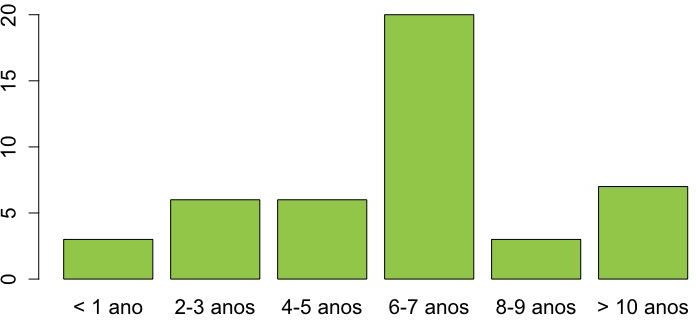
\includegraphics[width=.8\linewidth]{survey1-exp.jpg}
  \caption{Desenvolvimento de Software}
  \label{fig:sub1}
\end{subfigure}%
\begin{subfigure}{.5\textwidth}
  \centering
  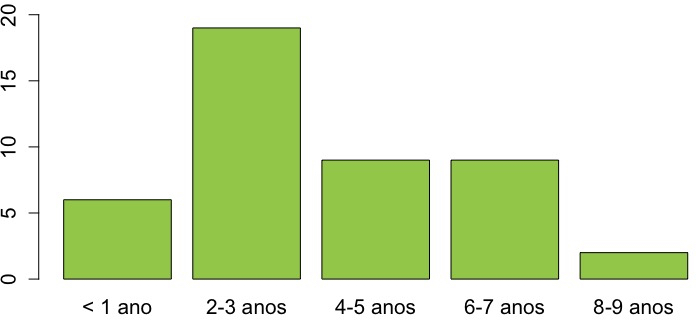
\includegraphics[width=.8\linewidth]{survey1-android-exp.jpg}
  \caption{Desenvolvimento Android}
  \label{fig:sub2}
\end{subfigure}
\caption{Experiência dos desenvolvedores em \textit{S1}.}
\label{fig:DadosDemograficos-Exp}
\end{figure*}

% \begin{table}[h]
% \centering
% \renewcommand*{\arraystretch}{1}
% \small
% \begin{tabular}{@{}l|c|r@{}}
% \toprule
% \textbf{Anos de Experiência} & \textbf{Participantes} & \multicolumn{1}{c}{\textbf{\%}}  \\
% \hline
% 1 ano ou menos 	&	 6 		& 	13,3 \%	 \\
% 2 anos 			& 	 7 		& 	15,6 \%	 \\
% 3 anos 			& 	 12		& 	26,7 \%	 \\
% 4 anos 			& 	 6 		& 	13,3 \%	 \\
% 5 anos 			& 	 3 		& 	 6,7 \%	 \\
% 6 anos 			& 	 7 		& 	15,6 \%	 \\
% 7 anos 			& 	 2 		& 	 4,4 \%	 \\
% 8 anos 			& 	 2 		& 	 4,4 \%	 \\
% \toprule
% \end{tabular}
% \caption{Experiência dos participantes com desenvolvimento Android.}
% \label{tab:DadosDemograficos}
% \end{table}

\subsubsection{Análise dos Dados}
\label{sub:smells-definition}

O processo de análise partiu da listagem das 45 respostas do questionário e se deu em 4 passos: verticalização, limpeza dos dados, codificação e divisão. \mau{encaixar o processo de análise com alguma literatura sobre o assunto, veja como a michaela também fez no paper dela ou meu paper no MSR desse ano (está no meu site).}

O processo que denominamos de \textit{verticalização} consistiu em considerar cada resposta de boa ou má prática como um registro individual a ser analisado. Ou seja, cada participante respondeu 18 perguntas sobre boas e más práticas no \textit{front-end} Android (2 perguntas para cada elemento e mais duas perguntas genéricas). Com o processo de \textit{verticalização}, cada uma dessas respostas se tornou um registro, ou seja, cada participante resultava em 18 respostas a serem analisadas, totalizando 810 respostas (18 perguntas multiplicado por 45 participantes) sobre boas e más práticas.

O passo seguinte foi realizar a \textit{limpeza dos dados}. Esse passo consistiu em remover respostas obviamente não úteis como respostas em branco, que continham frases como \textit{"Não"}, \textit{"Não que eu saiba"}, \textit{"Eu não me lembro"} e similares, as consideradas vagas como \textit{"Eu não tenho certeza se são boas praticas mas uso o que vejo por ai"}, as consideradas genéricas como \textit{"Como todo código java..."} e as que não eram relacionadas a boas práticas de código. Das 810 boas e más práticas, 352 foram consideradas e 458 desconsideradas. Das 352, 44,6\% foram apontadas como más práticas e 55,4\% como boas práticas. 

Em seguida, realizamos a codificação sobre as boas e más práticas. O processo de codificação consistiu em analisar cada resposta e atribuir uma ou mais categorias. Durante esse processo, houveram 30 respostas que não eram triviais de identificar uma categoria ou mesmo de dizer se essas respostas deveriam ser consideradas. Essas respostas foram marcadas como \textit{"talvez"} e reavaliadas ao final, onde 6 permaneceram e 24 foram desconsideradas. Ainda durante a codificação, 9 respostas incialmente consideradas, foram desconsideradas. Para toda resposta desconsiderada nesse passo, foi indicado um motivo. Ao final da codificação, as categorias foram agrupadas por temas.

Por último realizamos o passo de divisão. Esse passo consistiu em dividir as respostas que receberam mais de uma categoria em duas ou mais respostas, de acordo com o número de categorias identificadas, de forma a resultar em uma categoria por resposta. Por exemplo, a resposta \textit{"Não fazer Activities serem callbacks de execuções assíncronas. Herdar sempre das classes fornecidas pelas bibliotecas de suporte, nunca diretamente da plataforma"} indica na primeira oração uma categoria e na segunda oração, outra categoria. Ao dividí-la, mantivemos apenas o trecho da resposta relativo a categoria, como se fossem duas respostas distintas e válidas. Em algumas divisões realizadas, a resposta completa era necessária para entender ambas as categorizações, nesses casos, mantivemos a resposta original, mesmo que duplicada, e categorizamos cada uma de forma diferente. 

Ao final da análise constavam 389 respostas individualmente categorizadas sobre boas e más práticas no \textit{front-end} Android.




\subsection{Percepção dos Desenvolvedores}

Para responder a \textbf{QP2}, buscamos entender a percepção dos desenvolvedores sobre as quatro boas e más práticas classificadas com alta recorrência. Estes dados foram coletados através de um questionário online (\textit{S2}) respondido por 11 desenvolvedores Android. Nossas análises demonstram que de fato, códigos afetados pelas más práticas, são percebidos pelos desenvolvedores como códigos problemáticos.

\subsubsection{Questionário}
\label{sub:perception-survey}


O questionário foi composto por duas seções principais. A primeira objetivou coletar informações básicas sobre os antecedentes dos participantes e, em particular, sobre sua experiência (dados apresentados na Figura \ref{fig:survey2-exp}). Na segunda seção, os participantes foram solicitados a examinar seis códigos-fonte Android e, para cada uma deles, responder às seguintes perguntas: \\

\noindent
\textbf{Q1} Na sua opinião, este código apresenta algum problema de design e/ou implementação? (Sim/Não) \\

\noindent
\textbf{Q2} Se SIM, por favor explique quais são, na sua opinião, os problemas que afetam este código. (Resposta aberta) \\

\noindent
\textbf{Q3} Se SIM, por favor avalie a severidade do problema de design e/ou implementação selecionando dentre as opções a seguir um ponto. (Escala \textit{Likert} de 5 pontos indo de 1 -- muito baixo -- a 5 -- muito alto) \\

\noindent
\textbf{Q4} Na sua opinião, este código precisa ser refatorado? (Sim/Não) \\

\noindent
\textbf{Q5} Se SIM, como você faria esta refatoração? (Resposta aberta) \\

Os seis códigos apresentadas foram selecionadas aleatoriamente para cada participante de um conjunto de 58 códigos, contendo 24 códigos afetadas por uma das quatro más práticas Android de alta recorrência (seis para cada má prática), 10 códigos afetadas por cheiros de códigos tradicionais e 24 códigos limpos. Para reduzir viés, selecionamos apenas códigos relacionados ao \textit{front-end} Android definido no contexto deste artigo, ou seja: \textsc{Activities}, \textsc{Fragments}, \textsc{Adapters}, \textsc{Listeners}, \textsc{Styles}, \textsc{Strings}, \textsc{Drawables} e \textsc{Layouts}. Cada participante avaliou dois códigos selecionados aleatoriamente de cada um desses três grupos. Os 58 códigos foram aleatoriamente coletados de projetos Android de código aberto no GitHub.

Para reduzir o aprendizado e viés, cada participante recebeu os seis códigos selecionados aleatoriamente em uma ordem aleatória. Além disso, os participantes não estavam cientes de quais classes pertenciam a qual grupo (más práticas Android, cheiros de código tradicionais e limpo). Apenas foi dito que estávamos estudando qualidade de código em aplicações Android. Nenhum limite de tempo foi imposto para que eles concluíssem a tarefa.

\subsubsection{Participantes}
\label{sub:perception-participants}

\begin{figure*}
\centering
\begin{subfigure}{.5\textwidth}
  \centering
  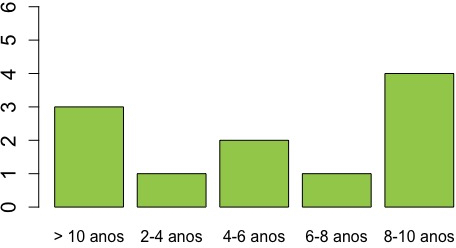
\includegraphics[width=.8\linewidth]{exp.jpg}
  \caption{Desenvolvimento de Software}
  \label{fig:sub1}
\end{subfigure}%
\begin{subfigure}{.5\textwidth}
  \centering
  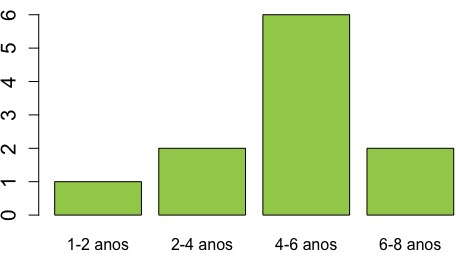
\includegraphics[width=.8\linewidth]{exp-android.jpg}
  \caption{Desenvolvimento Android}
  \label{fig:sub2}
\end{subfigure}
\caption{Experiência dos desenvolvedores em \textit{S2}.}
\label{fig:survey2-exp}
\end{figure*}


\subsubsection{Análise dos Dados}
\label{sub:perception-participants-analysis}

Para comparar as distribuições da gravidade indicada pelos participantes para os três grupos de classes, utilizamos o teste de Mann-Whitney não pareado [27] para analisar a significância estatística das diferenças entre a gravidade atribuída pelos participantes aos problemas que observam em MVC- Tradicional-smelly, e classes limpas. Os resultados são considerados estatisticamente significativos em alfa = 0,05. Também estimamos a magnitude das diferenças medidas usando o Delta de Cliff (ou d), uma medida de tamanho do efeito não paramétrico [49] para dados ordinais. Seguimos diretrizes bem estabelecidas para interpretar os valores do tamanho do efeito: insignificante para | d | menor 0,14, pequeno para 0,14 menor igual | d | menor 0,33, meio para 0,33 menor igual | d | menor 0,474, e grande para | d | maior igual 0,474 [49]. Finalmente, relatamos achados qualitativos derivados das respostas abertas dos participantes.

















